\documentclass[11pt]{article}
\usepackage{graphicx}
\usepackage{amssymb}
\usepackage{epstopdf}
\usepackage{rotating}
\usepackage{amsfonts}
\usepackage{natbib}
\usepackage{subfigure}
\usepackage{pdfsync}
\usepackage{xspace}
\usepackage{color}
\usepackage{url}
\usepackage{nameref}
%\usepackage[pdftex, colorlinks=true,urlcolor=blue]{hyperref}
%\usepackage{wallpaper}

%%%% HERE IS SOME WATERMARK STUFF
%\addtolength{\wpXoffset}{-.2in}
%\CenterWallPaper{1.1}{/Users/eriq/Documents/work/nonprj/WaterMarks/StrictDraftWatermark.eps}


\DeclareGraphicsRule{.tif}{png}{.png}{`convert #1 `dirname #1`/`basename #1 .tif`.png}

%% My baseurl.  Can be changed as necessary.


%% some handy things for making bold math
\def\bm#1{\mathpalette\bmstyle{#1}}
\def\bmstyle#1#2{\mbox{\boldmath$#1#2$}}
\newcommand{\thh}{^\mathrm{th}}


%% Some pretty etc.'s, etc...
\newcommand{\cf}{{\em cf.}\xspace }
\newcommand{\eg}{{\em e.g.},\xspace }
\newcommand{\ie}{{\em i.e.},\xspace }
\newcommand{\etal}{{\em et al.}\ }
\newcommand{\etc}{{\em etc.}\@\xspace}


\newcommand{\CR}{\mathrm{CR}}
\newcommand{\CWT}{\mathrm{CWT}}
\newcommand{\PBT}{\mathrm{PBT}}
\newcommand{\Var}{\mathrm{Var}}
\newcommand{\btheta}{\bm{\theta}}

%% the page dimensions from TeXShop's default---very nice
\textwidth = 6.5 in
\textheight = 9 in
\oddsidemargin = 0.0 in
\evensidemargin = 0.0 in
\topmargin = 0.0 in
\headheight = 0.0 in
\headsep = 0.0 in
\parskip = 0.2in
\parindent = 0.0in


\title{Assessing the potential for PBT to deliver \\
estimates currently obtained using CWTs: \\
a data-driven, large scale assessment}
\author{Eric C. Anderson\thanks{
    Fisheries Ecology Division, 
    Southwest Fisheries Science Center, 
    110 Shaffer Road,
    Santa Cruz, CA 95060}
}
\begin{document}

\maketitle

\tableofcontents

\section{Introduction}
Here, we seek to address this information need:
\begin{quote}
{\sl Assessment of the degree to which this [PBT] system could or could not deliver estimates of the key life history and fishery parameters that are currently delivered from the CWT program and do so with similar or better accuracy (i.e., consider errors of estimation). Identify areas or issues where implementation of PBT on a coast-wide basis seems most problematic. }
\end{quote}

There are two main variables that influence the accuracy of different estimates of life-history and 
fishery parameters obtained from CWT or PBT data: 1) the number of tags (CWT-based or PBT-based) that 
are actually recovered, and 2) the accuracy with which those tags can be expanded to meaningful estimates
of the expanded number of recoveries.  The main factor driving (2) is the accuracy with
which the tagging rate is known.  We deal with (2) in a separate document, ``Variation in
Parentage-Based Tagging and Coded-Wire  Tagging  Rates.''  In this document, we treat issue (1), assessing
the degree to which increasing tagging rates by using  PBT can improve
tag-recovery rates.  

Because tagging a higher fraction of any stock can be done cheaply with PBT, it is tempting to
think that increasing tagging rates using PBT will invariably lead to higher recovery rates
for all the release groups.  This is, however, untrue: it is necessary to mark (ad-clip) PBT-tagged
fish in order to recover them, and indiscriminately increasing the mark rate on numerous stocks
will almost certainly reduce the fraction of marked fish (in mixed fisheries) that originate from
certain weak or underrepresented stocks, decreasing the recovery rate for those stocks.  Therefore, 
increasing tag rates through PBT must be done in a more nuanced and selective fashion.  

The degree to which selective increases in mark and tagging rates can improve recovery rates for many 
stocks depends on a number of factors.  For example, recovery rates for a weak stock cannot be 
easily increased if that stock is already tagged and marked at 100\%.  Furthermore,
the effect upon any particular fishery of increasing the tagging and mark rates on a group of stocks depends
fundamentally upon the relative composition of those stocks in the fishery.  And, of course,
tag-and-mark-rate increases that improve recoveries of a release group that is rare in one fishery might,
if that stock is common in a second fishery, have the effect of reducing recovery rates of other
stocks in that second fishery.  On top of that, the effect of increasing tag rates on a fishery will
depend on other features of the fishery, for example, whether it is visually or electronically sampled.
Therefore, the potential for PBT to deliver improved estimates of fishery parameters on a coastwide scale
can only be answered by taking account of the stock composition of those fisheries and the sampling
schemes employed in them.  

Here, we divide the marine fisheries in the year 2012 for Chinook salmon along
the Pacific Coast of North America into
18 regions (recovery areas) and estimate the composition of fish recovered from those regions by applying a novel
Bayesian estimation model to data from the Regional Mark Information System (RMIS) data base.  After
confirming that the model fits the data well, we use the estimated composition of release groups
in each region to explore how expected recovery rates change under different scenarios of modified 
tagging and marking rates of PBT.  The expected recovery rates of PBT-tagged fish can be easily compared
to the expected recovery rates of CWTs given current tagging and marking rates, which provides a principled
way of assessing the degree to which a PBT program might be able to yield more recoveries, 
and hence more accurate estimates, from multiple release groups across the whole coast.   


The remainder of this document is divided into five main sections.  In {\sc \nameref{sec:prelims}},
we summarize and make explicit some of the assumptions and operating perspectives we have adopted
in this work.  {\sc \nameref{sec:bayes}} develops the  model used to estimate
proportions of different release groups in fisheries.  {\sc \nameref{sec:agg}} describes how we divided
Chinook fisheries in 2012 into a few large recovery areas and it gives a summary of the number of CWTs from
each release group recovered in those fisheries. In {\sc \nameref{sec:estimation}} we apply the
Bayesian model to each large recovery area and present the estimates, as well as the posterior
predictive checks which verify that the model fits the data.  Finally, in
{\sc\nameref{sec:compare}}, we discuss different schemes for setting tagging rates at
PBT hatcheries and then compare expected recovery rates under those schemes to the recovery
rates expected while using current CWT tagging rates.  





\section{Preliminaries and Assumptions \label{sec:prelims}}

In order to make this undertaking manageable, while still yielding useful information, we make several
assumptions, listed below:
\begin{enumerate}
\item {\sl The tag-code is the basic unit for fishery estimation.} We suspect that for many estimation purposes
it is customary to aggregate multiple tag-codes (release groups) from a given hatchery or across multiple
hatcheries in a single stock, but we have not done that here.  Our estimates of fishery proportions will
always be with respect to different tag codes.  Since there are so many tag codes, and many release groups
are rather small, a consequence of this is that it is not possible to obtain accurate estimates of proportions
without large samples.
\item {\sl Fishery samples across nearby locations and over time can be aggregated. } In order to investigate
recovery areas in which a sufficient number of tags are recovered to make meaningful estimates
of the proportion of numerous small release groups, we aggregate somewhat aggressively over space and time. 
Obviously, fishery composition varies spatially and temporally; however, our purpose here is not to estimate
proportions for any single small fishery.  Rather we want to get reasonable estimates of composition across
several large swaths of coast, so as to represent the range of compositions one might encounter 
coastwide.  
\item {\sl The tagged and marked fractions of a release group are constant over the life of the fish.}  This
assumption would be violated if marked or tagged fish experience higher mortality than their unmarked
counterparts, as could be the case in the presence of very strong mark-selective fishing pressure.  Trying to
account for this, however, does not seem relevant to our task. Keep in mind that, we are interested in
getting estimates of fishery compositions that might reasonably be encountered---we are not trying to accurately
estimate the composition in any specific fishery.
\item {\sl The only type of mark we concern ourselves with in the estimation of proportions is the
adipose clip.}  An adipose clip in conjunction with another mark is counted simply as an ad-clip.
\item {\sl In this document we do not directly address the suitability of either PBT or CWTs for doing DIT-based estimation.}
\item {\sl We are developing these methods in the context of recoveries from fisheries, but they could easily be
extended to escapement, \etc}
\end{enumerate}


\section{Bayesian Estimation of Release Group Proportions \label{sec:bayes}}

We propose a simple model to estimate the composition of fish from different release groups,
using CWT recovery data.  We then specify a Gibbs sampler to sample from the posterior
distribution of the parameters in the model.

\subsection{Model for Visually-Sampled Fisheries}

We first formulate the model for visually-sampled fisheries.  It is subsequently
relatively straightforward to extend it
to electronically-sampled fisheries.


\subsubsection{Parameters}

Let $\theta_g$ be
the probability that a fish sampled 
from the ocean within a given recovery area  is from release group $g$, $g = 1,\ldots, G$,
where $G$ is the total number of distinct tag codes with at least one recovery, coastwide,
during the year.  Denote all of those probabilities by $\btheta = (\theta_1, \ldots, \theta_G)$.
We don't specifically denote the recovery area in order to avoid an
overproliferation of subscripts, but remind the reader that $\theta_g$ is defined in
reference to a particular recovery area. Note that $\btheta$ might not reflect the
true composition of fish in the recovery area because of length restrictions on the catch, \etc  We contend
that this is not a great concern because, for our purpose, what we wish to estimate is the
probability that a fish from a certain release group will
be caught and retained in the fishery, and that is precisely what $\theta_g$ reflects.


We define each release group, $g$, to correspond explicitly to a tag code; however, it is important
to understand that $\theta_g$ refers not just to the fraction of fish from release group $g$ that
have CWTs, but {\em all} of the fish in the release group $g$, whether they have
a CWT (or an ad-clip) or not. As stated above, 
we think of tag codes, $g$, as being indexed from 1 up to $G$ for the $G$ distinct tag {\em codes}
(not tags, themselves)
that were actually observed in at least one marine fishery during the given year. 


Our model includes four more categories to which a fish that is not from a release group may belong:
\begin{description}
\item{$A+$ and $A-$:}~~Fish from non-associated release groups that carry agency-only or blank wire.  These fish cannot be identified to release group but they do all carry wire. The $+$ and the $-$ refer to whether or
not the fish is ad-clipped.
\item{$U+$ and $U-$:}~~Fish that don't carry wire of any sort and are not part of an associated release group.  If
they have an ad-clip, they are part of $U+$; if they don't, they are part of $U-$.  Untagged and unmarked wild
fish are part of $U-$, as are unmarked fish from non-associated releases.  Untagged but marked fish from
non-associated releases are in $U+$.  When we say ``associated release group'' we are referring specifically
to a tagged release record with a {\tt record\_code} of ``T'' in the RMIS Release Data Base.  We use the phrase
``non-associated'' release to mean a hatchery release that would be denoted in the Release Data Base with
{\tt record\_code} ``N'' (or any other release that might not have been recorded in the data base at all).
\end{description}
Some portions of the $A$ and $U$ categories are not likely to be easily estimated,
as they represent the ``leftover'' after all
the fish from associated releases are accounted for. 

The parameters in the model we are interested in estimating are collectively denoted
\[
\btheta = (\theta_{A+}, \theta_{A-}, \theta_{U+}, \theta_{U-},\theta_1,\ldots,\theta_{G})
\] 
and we note that 
\[
\theta_{A+} + \theta_{A-} + \theta_{U+} + \theta_{U-} + \sum_{g=1}^{G} \theta_g = 1.
\] 
We will assume a Dirichlet prior on these probabilities parameterized by the vector
$\bm{\gamma} = (\gamma_{A+},\- \gamma_{A-},\- \gamma_{U+},\- \gamma_{U-},\- \gamma_{1}, \ldots, \gamma_G)$, so that 
{\em a priori}
\[
\btheta \sim \mathrm{Dirichlet}(\bm{\gamma}).
\]
We use $\gamma_{A+} = \gamma_{A-} = \gamma_{U+} = \gamma_{U-} = \frac{1}{4}$ and $\gamma_g = \frac{1}{G}$, for $g=1,\ldots, G$.



\subsubsection{Release, Catch-Sample, and Recovery Data}

In each tagged release group $g$, a fraction $f^{(m)}_g$ ($0\leq f^{(m)}_g \leq 1$)
of the fish in the release group are marked,
and the remainder (a fraction $1-f^{(m)}_g$) are unmarked. We consider a fish to be 
``marked'' if it has an ad-clip (whether or
not in combination with another mark).   Associated with both the marked and unmarked
fractions is a CWT tagging rate.  The variable $p^{(m)}_g$ denotes the
fraction of the marked fish from release group $g$ that carry CWTs, and $p^{(u)}_g$ denotes the fraction
of unmarked fish from release group $g$ that carry CWTs. Both $p^{(m)}_g$ and  $p^{(u)}_g$ are between
0 and 1, inclusive; however they needn't necessarily sum to 1.  For each $g=1,\ldots,G$, the value of
$f^{(m)}_g$, $p^{(m)}_g$, and $p^{(u)}_g$ can be obtained
from the RMIS release data base.

For each recovery area, we provide the model with $N_v$---the number of fish that were
visually sampled for adipose fin clips.  $N_v$ can be found by summing the {\tt mr\_1st\_sample\_known\_ad\_status} field in the RMIS catch-sample data base across all the fisheries in the recovery area over the
time in question.  

\subsubsection{The Data (Missing and Otherwise) for Each Sampled Fish}
We develop our estimation framework by noticing that we are missing information
that would make the estimation problem quite easy---namely, if we knew the release group of every
fish we sampled in a fishery (whether it had a CWT or an ad-clip or not).  In that case, we would have a simple multinomial
formulation with a Dirichlet prior.  Of course, we don't know the release group of every sampled
fish---that information is missing!  However, thinking about the problem this way shows us that it is a classic
missing-data problem for which the EM-algorithm or Gibbs sampling are useful.  In our case we will
formulate a way to sample over the unknown origins of all of the sampled fish in a stratum whose release group
is not known, given 
everything else we know about them.
In other words, for every fish that is handled in some way (either visually inspected for an ad-clip or,
when we extend the model below,
electronically scanned for a CWT) we can sample over that crucial piece of missing data---the fish's origin.
Having sampled all the fish's tag-codes of origin we can use them to update our estimate of
$\btheta$, and then iterate that process---a simple Gibbs sampler that will be described in detail below.


For each fish that is sampled---any fish that someone looks at to see if it has an ad-clip---the list below shows what we shall keep track of (and
update/impute as necessary).  The names in {\tt monospaced} font below refer to the specifications that
will be used in the computer code that goes with this project, and the mathematical notations immediately
following give
the indicator variables and their values that will be used in the upcoming mathematical formulations.
Values corresponding to ``unobserved''  
are colored blue. Those are values that will be udpated during the course of MCMC.
\begin{description}
	\item [{\tt ad\_clipped}:]  ~~~$\delta_i^{(\mathrm{ac})}$~~~Does the fish have an adipose clip? 	An ad-clip, even in combination with any other marks is still counted.
	\begin{description}
		\item [{\tt yes}:]  ~~~$\delta_i^{(\mathrm{ac})} = 1$~~~The fish was observed to have an ad-clip.
		\item [{\tt no}:]  ~~~$\delta_i^{(\mathrm{ac})} = 0$~~~The fish was observed to {\em not} have an ad-clip.
		\item [\textcolor{blue}{{\tt unknown}}:]  ~~~$\delta_i^{(\mathrm{ac})} = \mbox{?}$~~~The fish was either not
		inspected for a mark, or it was and its mark status was ambiguous.
	\end{description}
	\item [{\tt cwt\_status}:] ~~~$\delta_i^{(\mathrm{cs})}$~~~Does the individual carry a CWT or not, and what category of wire is
	it? (this is {\em not} the same as the tag code of the fish).
	\begin{description}
		\item [{\tt cwt}:] ~~~$\delta_i^{(\mathrm{cs})} = 1$~~~The fish is known to carry a coded wire tag, and it
		was read appropriately.
		\item [{\tt no\_read}] ~~~$\delta_i^{(\mathrm{cs})} = n$~~~This corresponds to all fish that
		are observed to have a non-agency-only CWT but which is not readable, or was apparently read incorrectly.  This 
		includes the categories ``Tag lost before read,'' ``Tag not readable,'' 
		and ``Unresolved discrepancy.''
		\item [{\tt awt}:] ~~~$\delta_i^{(\mathrm{cs})} = a$~~~Agency-only or blank wire.
		\item [{\tt no\_tag}:] ~~~$\delta_i^{(\mathrm{cs})} = 0$~~~The fish is observed to {\em not} carry a CWT
		\item [\textcolor{blue}{{\tt unknown}}:] ~~~$\delta_i^{(\mathrm{cs})} = \mbox{?}$~~~It is unknown if the fish carried a CWT or not.  This would be the case, for example
		in fish that had an ad-clip but were not assessed for the presence of a CWT, or fish that did not have
		an ad-clip and were not assessed for the presence of a CWT.
	\end{description}
	\item [{\tt tag\_code}:] ~~~$\delta_i^{(\mathrm{tc})}$~~~What is the tag code that corresponds to the release group that the fish comes from.
	\begin{description}
		\item [{\tt code}:] ~~~$\delta_i^{(\mathrm{tc})} = g$~~~Whatever the tag code is for the release group the fish was a part of.  In fish without CWTs, this value will not be directly known, but we can still think of each
		fish as having an origin.
		use $g$ to index these tag codes.
		\item [\textcolor{blue}{{\tt unknown}}:] ~~~$\delta_i^{(\mathrm{tc})} = \mbox{?}$~~~This is the starting value
		for anything that is a {\tt no\_read}.
		\item [\textcolor{blue}{{\tt pending}}:] ~~~$\delta_i^{(\mathrm{tc})} = p$ ~~~~ This is the value we give things
		that have unknown cwt status.  
		\item [{\tt irrelevant}:] This is the case if {\tt cwt\_status} is not {\tt cwt}, {\tt no\_read}, or {\tt unknown}.  
	\end{description}
\end{description}




\subsubsection{Probabilities of Fully-Observed Categories}
Given the current value of $\btheta$, it is straightforward to compute the expected proportions of fish
in the six fully-observed categories corresponding to the two possible observed states of ad-clipping, 
$\delta_i^{(\mathrm{ac})} = 1$ and $\delta_i^{(\mathrm{ac})} = 0$, and the 3 possible states of CWT status:
1) the fish is known to have a CWT: either $\delta_i^{(\mathrm{cs})} = 1$ or $\delta_i^{(\mathrm{cs})} = n$, 2) the fish
is known to have agency-only wire: $\delta_i^{(\mathrm{cs})} = a$, or 3) the fish is known to carry no wire at all:
$\delta_i^{(\mathrm{cs})} = 0$. These probabilities, enumerated in Table~\ref{tab:probs}, provide us with the values
we need for computing the full conditional distribution of the ad-clip status and {\tt cwt-status} of every sampled individual
that is not fully observed for those characteristics.
\begin{table}
\caption{Expected fractions (probabilities) of fully-observed categories given $\btheta$.  The ``Symbol'' column shows
how we will subsequently refer to each of these probabilities. \label{tab:probs} }
\begin{center}
\begin{tabular}{lcccl}
\hline \hline\\
Category&~~~~~$\delta_i^{(\mathrm{ac})}$~~~~~      &      ~~~~~$\delta_i^{(\mathrm{cs})}$~~~~~     &     ~~~~~Symbol~~~~~   &   Probability \\\hline
\\
1 & 1 &  1 or $n$  &  $\phi_{1,1}$     &  $\sum_{g=1}^G \theta_g f_g^{(m)}  p_g^{(m)}$ \\
\\
2 & 1 &  $a$  &  $\phi_{1,a}$     &  $\theta_{A+}$ \\ 
\\
3 & 1 &  0  &  $\phi_{1,0}$     &  $\sum_{g=1}^G \theta_g f_g^{(m)}  (1 - p_g^{(m)}) + \theta_{U+}$  \\
\\
4 & 0 &  1 or $n$  &  $\phi_{0,1}$     &  $\sum_{g=1}^G \theta_g (1 - f_g^{(m)})  p_g^{(u)}$ \\
\\
5 & 0 &  $a$  &  $\phi_{0,a}$     &  $\theta_{A-}$ \\ 
\\
6 & 0 &  0  &  $\phi_{0,0}$     &  $\sum_{g=1}^G \theta_g  (1 - f_g^{(m)}) (1 - p_g^{(u)}) + \theta_{U-}$  \\
\hline\hline
\end{tabular}
\end{center}
\end{table}
For example, a fish that had unknown ad-clip status and unkown {\tt cwt\_status} could belong to any of categories~1--6,
and the full conditional probability that it belongs to any of those is given by the probabilities $\phi_{1,1},\ldots,\phi_{0,0}$, respectively.  By contrast, for example, a fish that was known to have
an ad-clip, but had unknown {\tt cwt\_status} could
only belong to one of the three fully observed categories~1--3, each with probability proportional to $\phi_{1,1}$, 
$\phi_{1,a}$, or $\phi_{1,0}$.

An important summary of the data is the number of sampled fish in each category.  We let $n_{1,1}$ denote the number 
of sampled fish that are known to have an ad-clip and are known to have a CWT.  Likewise, $n_{1,a}$, $n_{1,0}$, $n_{0,1}$, $n_{0,a}$, and $n_{0,0}$ are defined in a similar fashion with their subscripts corresponding to the $\phi$ 
symbols of Table~\ref{tab:probs}. The collection of a all of these $n$'s, summarized in vector form we refer to as $\bm{n} =
(n_{1,1}, n_{1,a}, n_{1,0}, n_{0,1}, n_{0,a}, n_{0,0})$. Finally, fish with unknown ad-clip or CWT status are counted yielding $n_{1,?}$ fish with
an ad-clip but with unknown {\tt cwt\_status}; $n_{0,?}$ fish known to have no ad-clip but with unknown {\tt cwt\_status}; $n_{?,1}$ fish with unknown ad-clip status that have coded wire tags; $n_{?,a}$ fish with unknown ad-clip status that are known to have agency-only wire; $n_{?,0}$ fish with unknown ad-clip status
that are known to not have coded wire tags; and $n_{?,?}$ fish with unknown ad-clip and CWT status.

\subsubsection{MCMC}

Given this setup, we devise a straightforward Gibbs sampler that samples values of $\btheta$, and the 
{\tt unknown} variables for each sampled fish from their joint posterior distribution. Each sweep of the MCMC
algorithm simply involves sampling from a few multinomial distributions.  Given a current value of $\btheta$, the
algorithm proceeds as follows:
\begin{enumerate}
\item {\em Allocate the $n_{?,?}$ fish to ad-clipped and non-adclipped categories with or without CWTs:} The $n_{?,?}$ fish are simulated into
imputed ad-clip and CWT-status categories by drawing from their full conditional:
\[
\bm{m}^{(1)} = 
(m^{(1)}_{1,1}, m^{(1)}_{1,a}, m^{(1)}_{1,0}, m^{(1)}_{0,1},  m^{(1)}_{0,a},  m^{(1)}_{0,0}) \sim 
\mathrm{Mult}_6\biggl(n_{?,?}\, ; \,(\phi_{1,1}, \phi_{1,a}, \phi_{1,0}, \phi_{0,1}, \phi_{0,a}, \phi_{0,0})\biggr).
\] 
\item Allocate the $n_{?,1}$ fish to categories in which their unknown ad-clip status has been imputed:
\[
\bm{m}^{(2)} = 
(m^{(1)}_{1,1}, 0, 0, m^{(1)}_{0,1},  0,  0) \sim 
\mathrm{Mult}_6\biggl(n_{?,1}\, ; \,(\phi_{1,1}, \phi_{0,1}) / (\phi_{1,1} + \phi_{0,1})\biggr).
\]
\item {\em And so forth\ldots}  Similar, easily-derived, update rules are applied to allocate the $n_{?,a}$, $n_{?,0}$, 
$n_{1,?}$, and $n_{0,?}$, fish in the sample into vectors $\bm{m}^{(3)}$, $\bm{m}^{(4)}$, $\bm{m}^{(5)}$, and $\bm{m}^{(6)}$, 
respectively. 
\item The fully-observed and imputed individuals whose release group is unknown 
(because, for example, their tag was unreadable or 
ambiguous, or because they had no tag) 
are allocated to a release group, or to one of the groups $A+$, $A-$, $U+$, or $U-$, by sampling from 
cell probabilities that are computed 
by appropriate weightings of $\btheta$. For example, fish known (or imputed) to have an ad-clip and a coded
wire tag, but with unknown or unreadable tag code are allocated to the $G$ categories with cell probabilities equal to
\[
p_g =  \frac{\theta_g f_g^{(m)}  p_g^{(m)}}
{\sum_{g=1}^G \theta_g f_g^{(m)}  p_g^{(m)}}.
\]
Or, for another example, fish known (or imputed) to have no ad-clip and no wire in them are allocated to the $G$ groups or to
the $U-$ category by sampling from a multinomial with the following cell probabilities:
\begin{eqnarray}
p_{U-} & = &  \frac{\theta_{U-}}{\sum_{g=1}^G \theta_g  (1 - f_g^{(m)}) (1 - p_g^{(u)}) + \theta_{U-}} \\
p_{g} & = &  \frac{\theta_{g}}{\sum_{g=1}^G \theta_g  (1 - f_g^{(m)}) (1 - p_g^{(u)}) + \theta_{U-}}~~~,~~~g = 1,\ldots, G \\
\end{eqnarray}
\item Once a tag code or $A+$, $A-$, $U+$, or $U-$ is either known or has been imputed for every sampled fish, we count up
the number of fish in each category, $\bm{z} = (z_{A+},\- z_{A-},\- z_{U+},\- z_{U-},\- z_{1}, \ldots, z_G)$,
and finally we draw $\btheta'$, an updated value of $\btheta$, by sampling from a Dirichlet distribution:
\[
\btheta' \sim \mathrm{Dirichlet}(\bm{\gamma} + \bm{z})
\]
\item Set $\btheta$ to $\btheta'$, recalculate the $\phi$ values in Table~\ref{tab:probs}, and then return to step~1 above.
\end{enumerate}








\subsection{Extension to Electronically Sampled Fisheries}


To do so we will
introduce one more parameter whose value will be estimated from the data:  $\alpha$, the probability
of a false-positive beep.  $\alpha$ is the probability that a fish carrying no wire still gets a positive
beep during electronic detection.  We will assume that the false-negative rate for electronic detection is
negligible.




\begin{description}
	\item [{\tt detection\_method}:] ~~~$\delta_i^{(\mathrm{dm})}$~~~The method used to screen fish to discover CWTs. ($\delta_i^{(\mathrm{dm})}$ is the detection method of fish $i$ in the sample).
	\begin{itemize}
		\item [{\tt V}:] ~~~$\delta_i^{(\mathrm{dm})} = \mathrm{V}$~~~if the fish was visually sampled.
		\item [{\tt E}:] ~~~$\delta_i^{(\mathrm{dm})} = \mathrm{E}$~~~if the fish was electronically sampled.
	\end{itemize}
	\item [{\tt beep}:] ~~~$\delta_i^{(\mathrm{b})}$~~~Whether or not it beeped upon electronic detection. Possible values are:
	\begin{description}
		\item [{\tt yes}:] ~~~$\delta_i^{(\mathrm{b})} = 1$~~~The fish beeped when detected electronically.
		\item [{\tt no}:]  ~~~$\delta_i^{(\mathrm{b})} = 0$~~~The fish did not beep when detected electronically.
		\item [{\tt irrelevant}:] The fish was not sampled electronically.
		Must be irrelevant if detection\_method is {\tt V}. Might be irrelevant if the fish is part of a
		mark sample that is drawn {\em independently} of the beep-status for fish in a fishery with
		electronic detection.
	\end{description}

\end{description}

\section{Aggregation and Characterization of 2012 Fisheries \label{sec:agg}}

\begin{sidewaysfigure}
\begin{center}
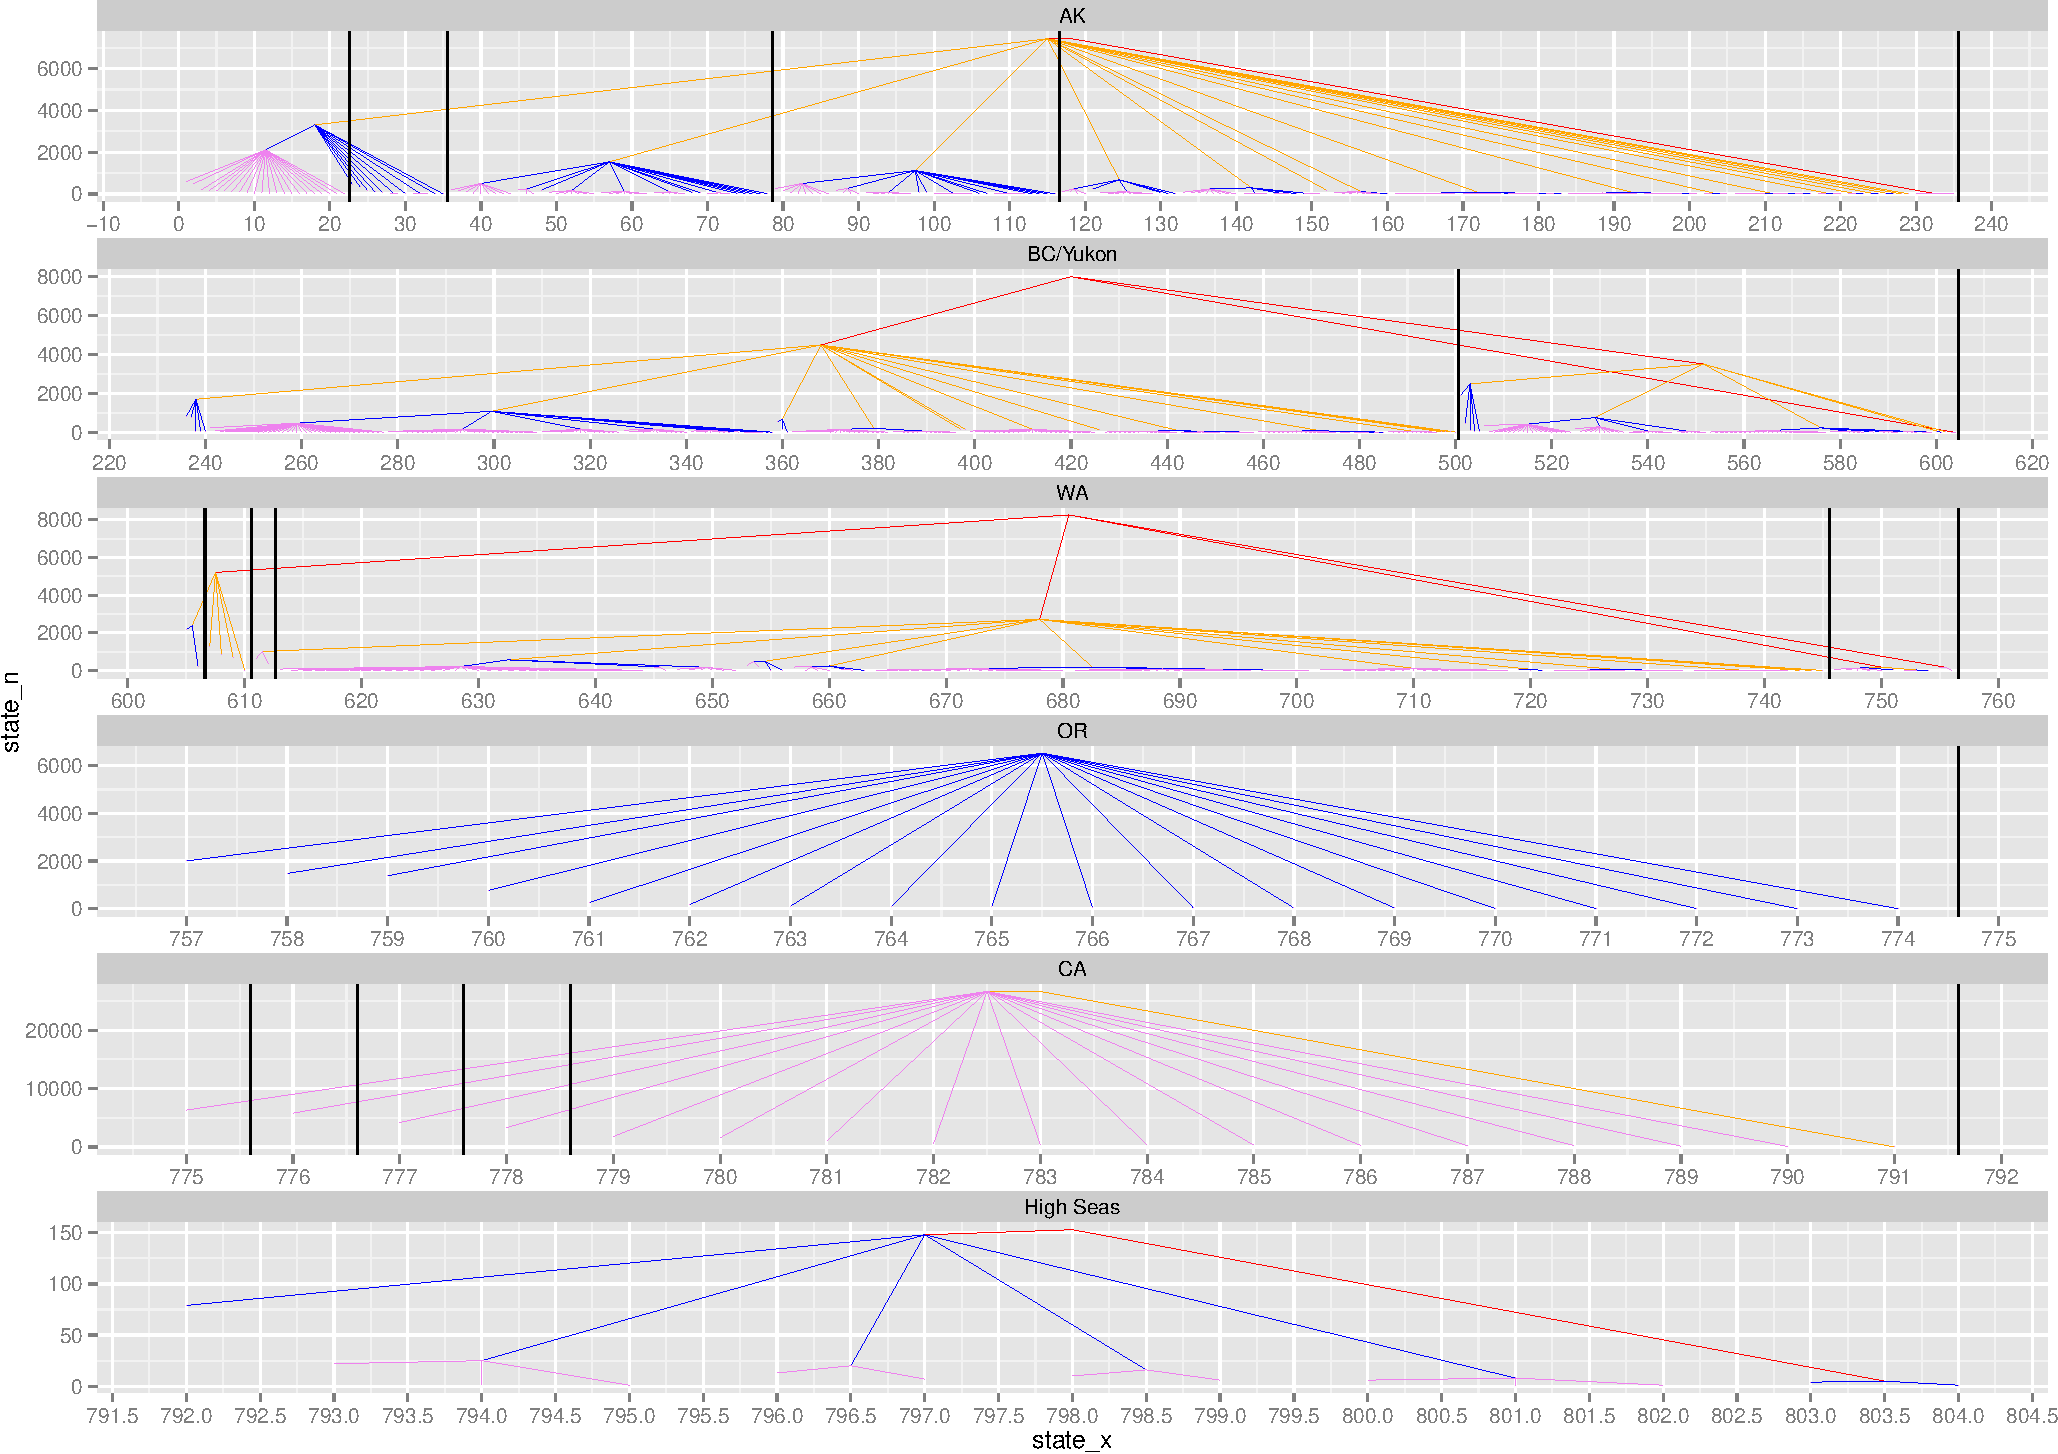
\includegraphics[width=\textwidth]{images/recovery_trees_divided.pdf}
\end{center}
\caption{Visual depiction of the hierarchical clustering of fishery recovery areas (and numbers of CWTs recovered)
in 2012.}
\end{sidewaysfigure}


\begin{sidewaysfigure}
\begin{center}
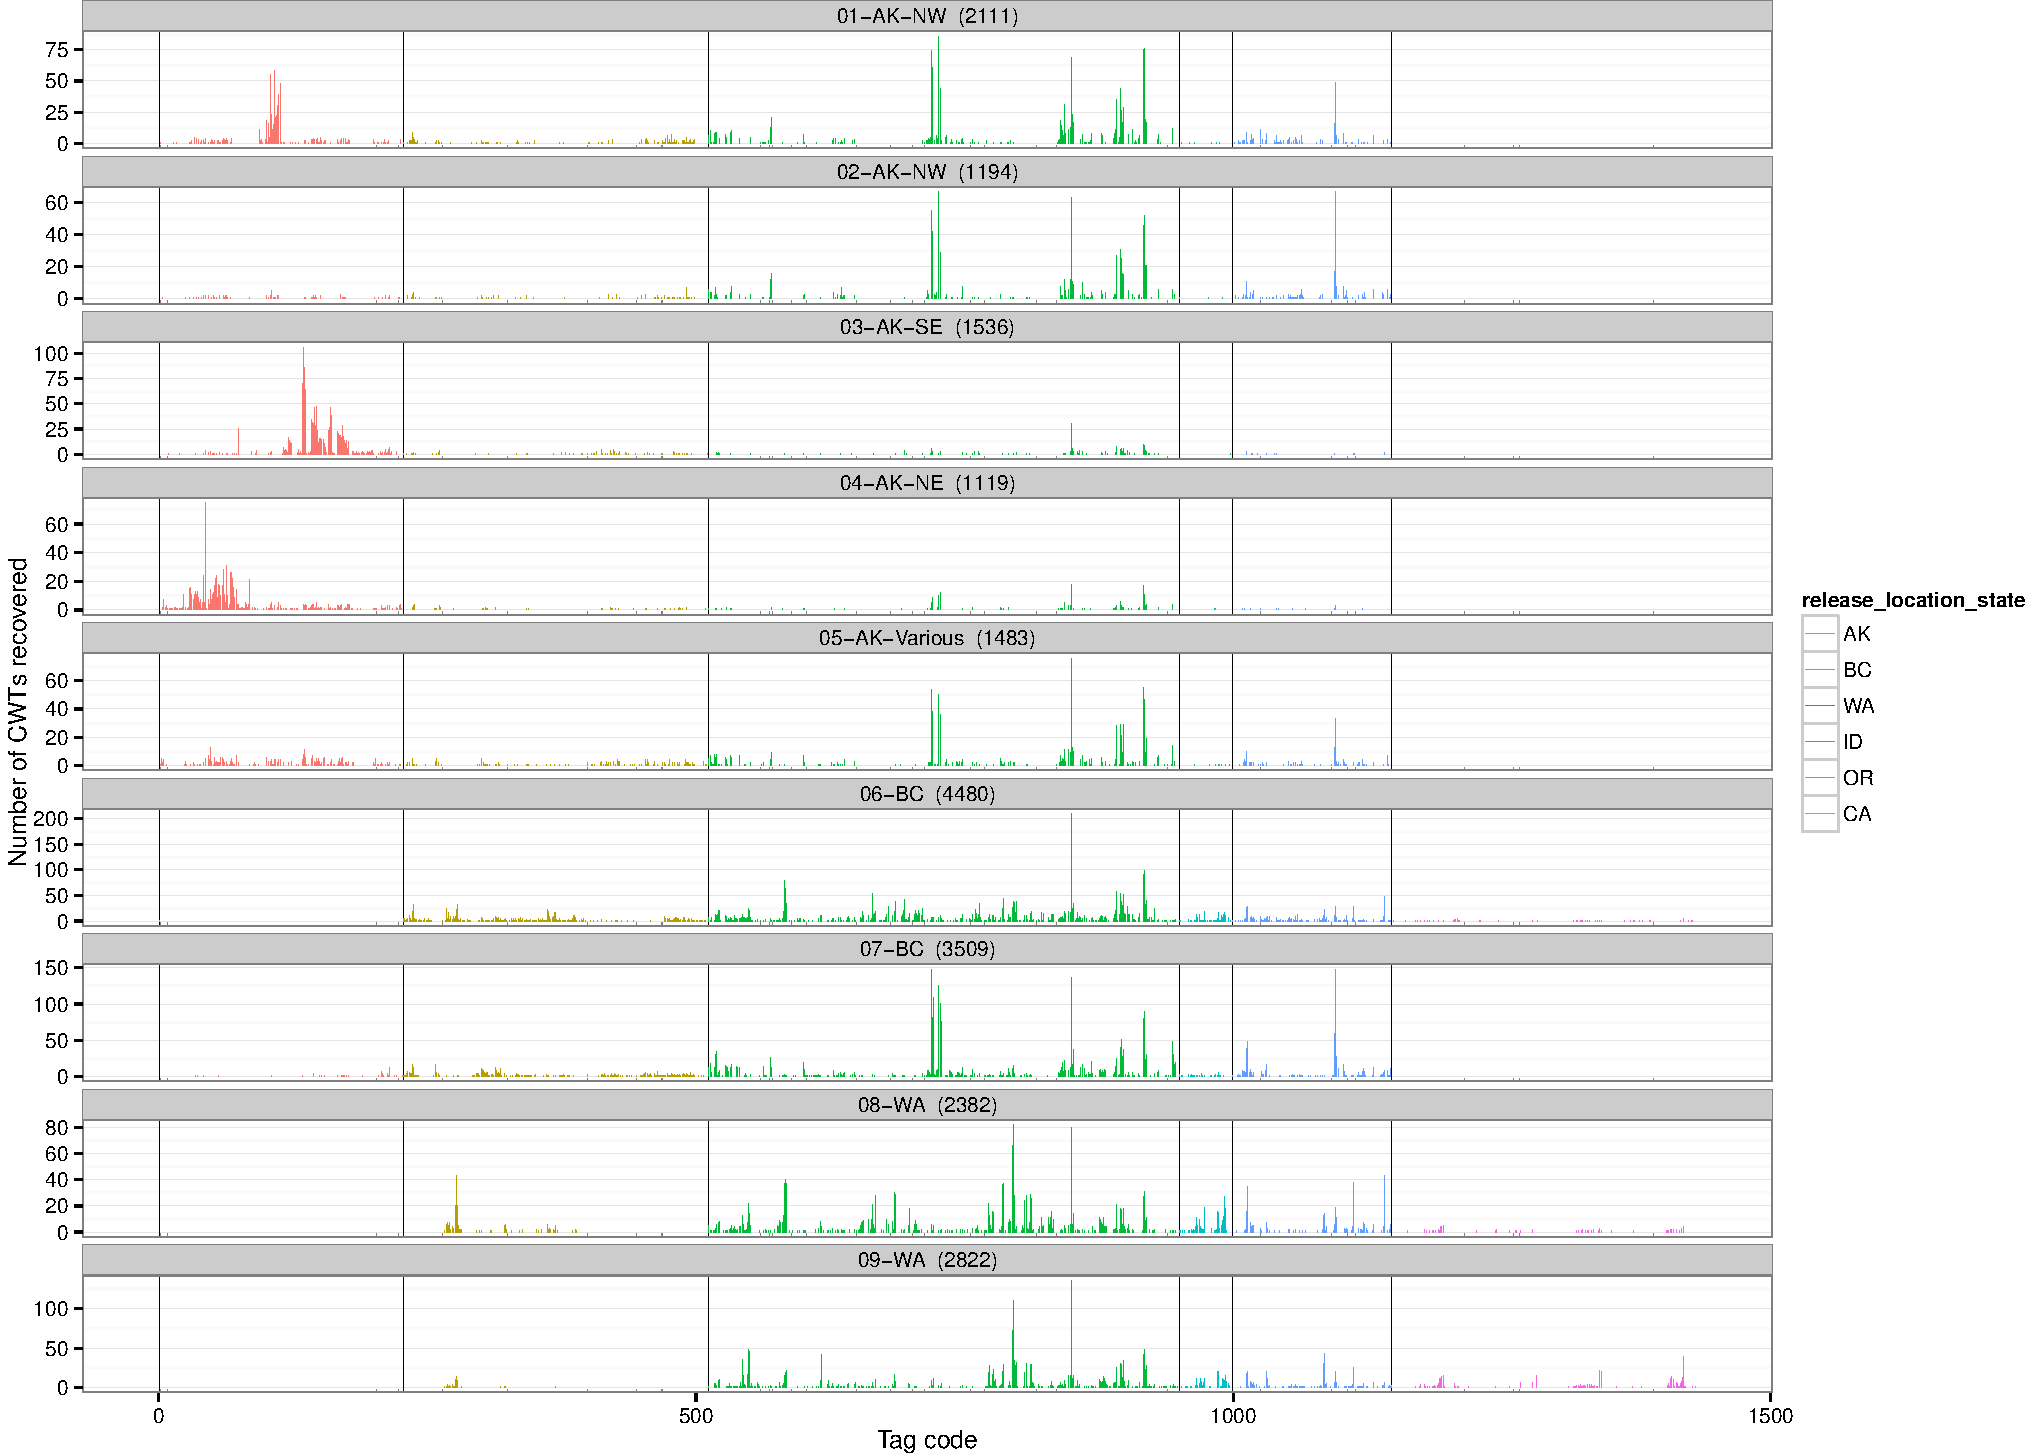
\includegraphics[width=\textwidth]{images/recovery_histo_panel_1.pdf}
\end{center}
\caption{The number of CWT recoveries from 1435 Chinook tag codes across different recovery areas in 2012, from Alaska to Washington.}
\end{sidewaysfigure}


\begin{sidewaysfigure}
\begin{center}
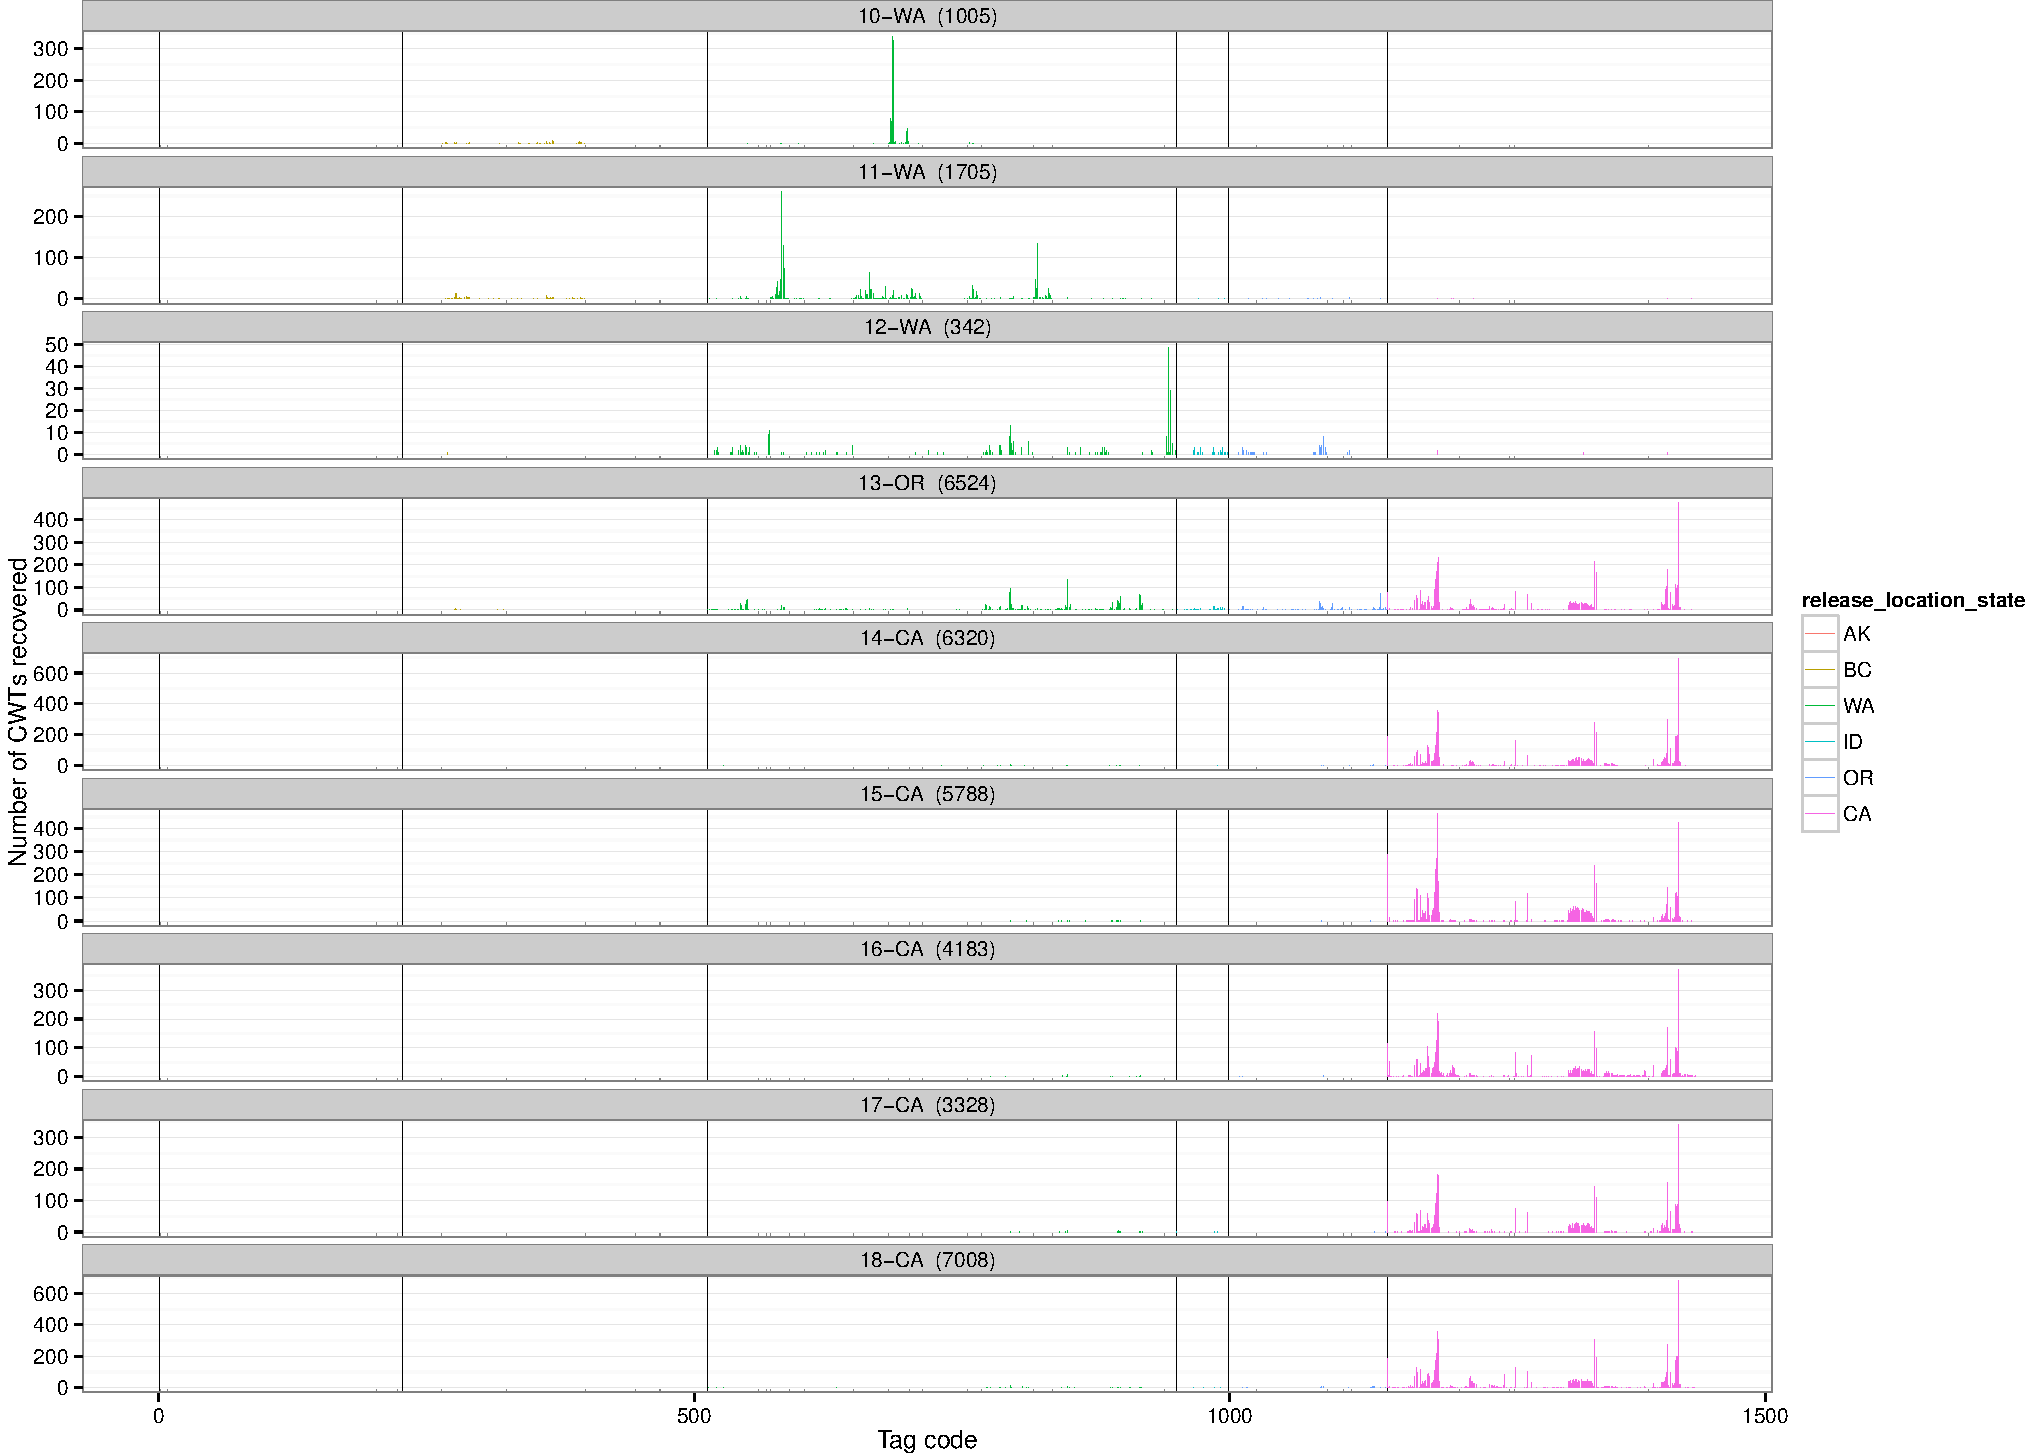
\includegraphics[width=\textwidth]{images/recovery_histo_panel_2.pdf}
\end{center}
\caption{The number of CWT recoveries from 1435 Chinook tag codes across different recovery areas in 2012, from Washington to California.}
\end{sidewaysfigure}


\section{Estimation of $\btheta$ in Fisheries Along the Coast \label{sec:estimation}}

\begin{sidewaysfigure}
\begin{center}
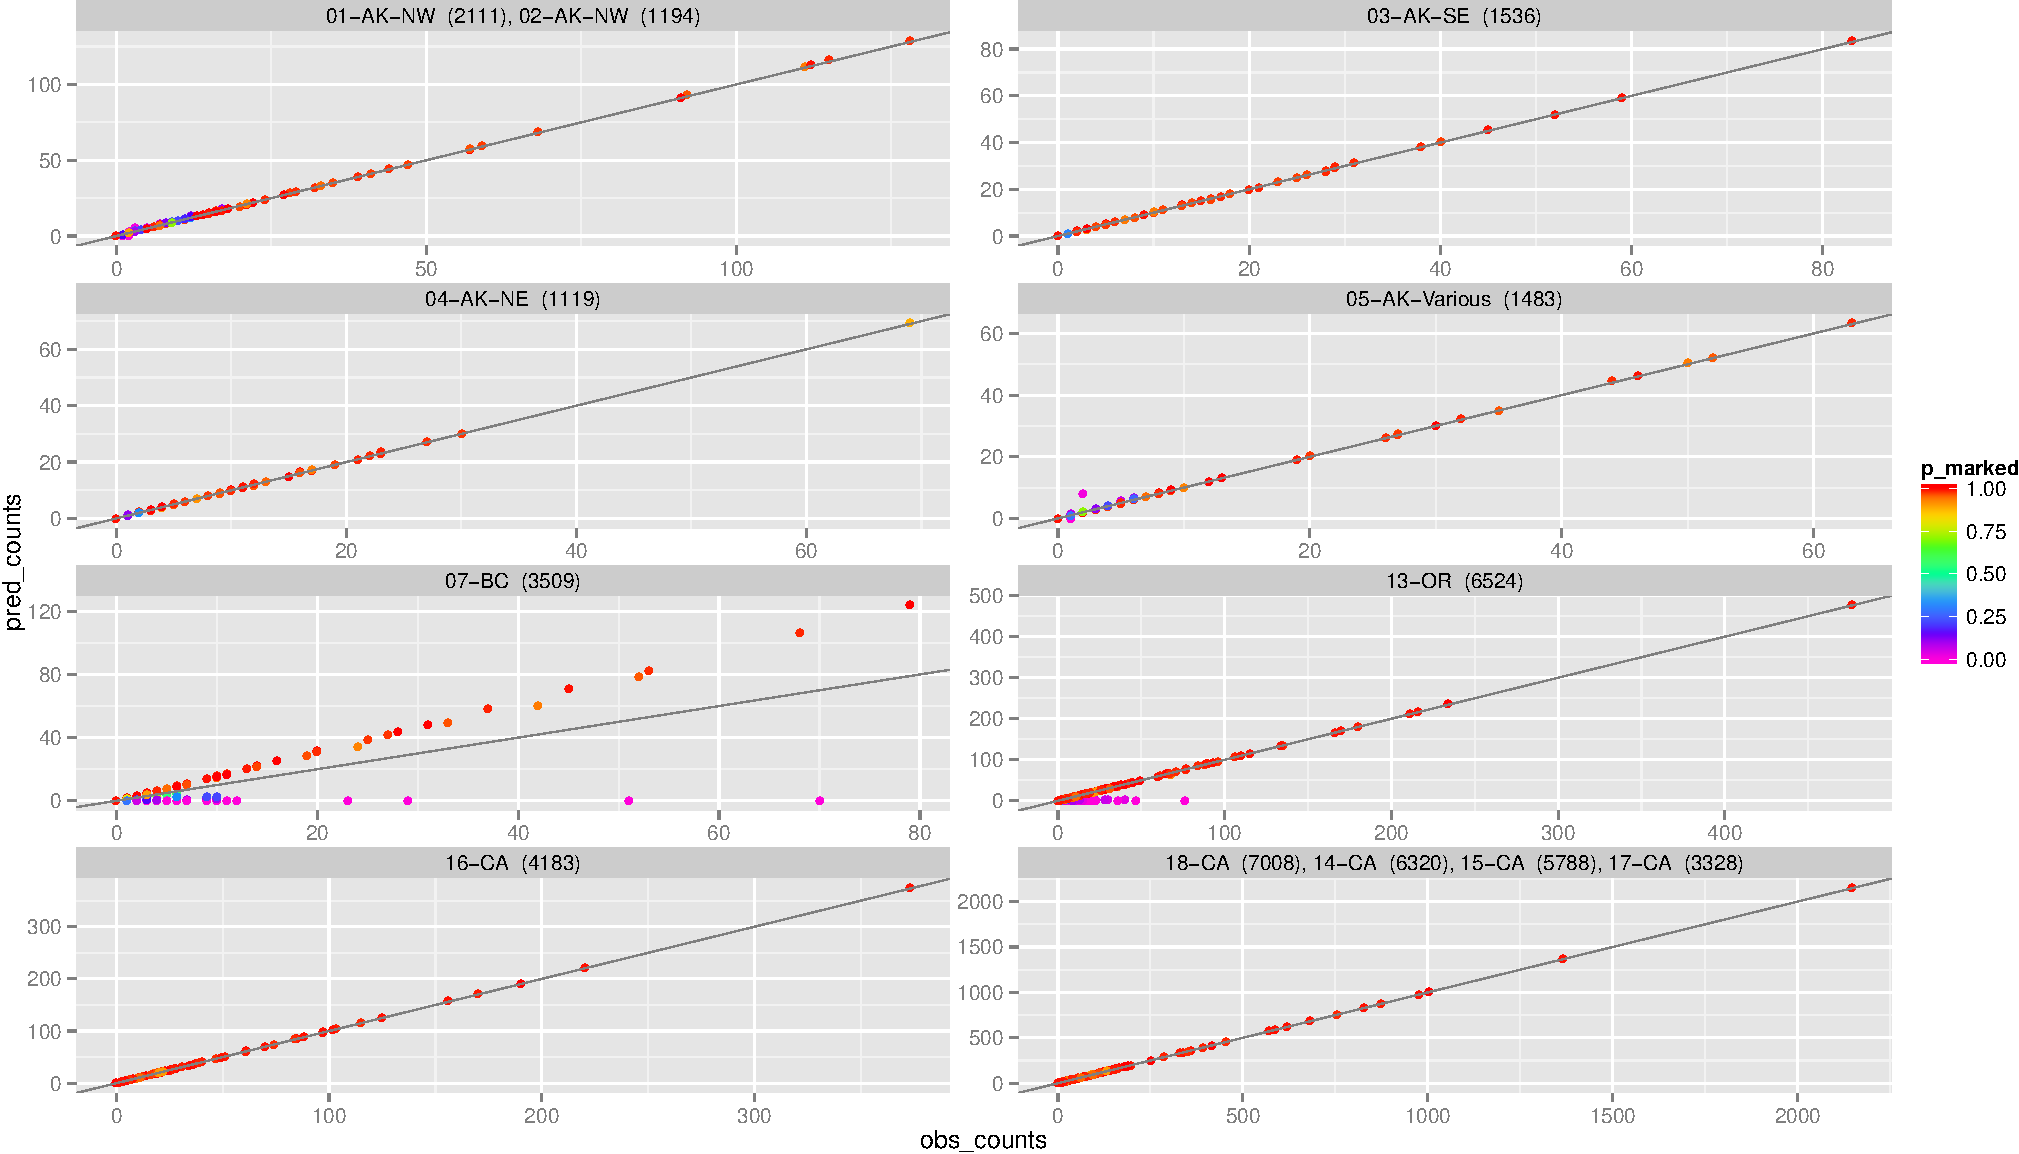
\includegraphics[width=\textwidth]{images/actual_vs_pred_cwt_recoveries_p_marked.pdf}
\end{center}
\caption{Posterior predictive checks of the the number of CWT recoveries predicted from the parameter estimates compared
to the actual number of recoveries.  Each point is a tag code which is colored according to $p_m$.  Note that occurrence
of BC release groups with $p_m$ reported to be 0.}
\end{sidewaysfigure}



\begin{sidewaysfigure}
\begin{center}
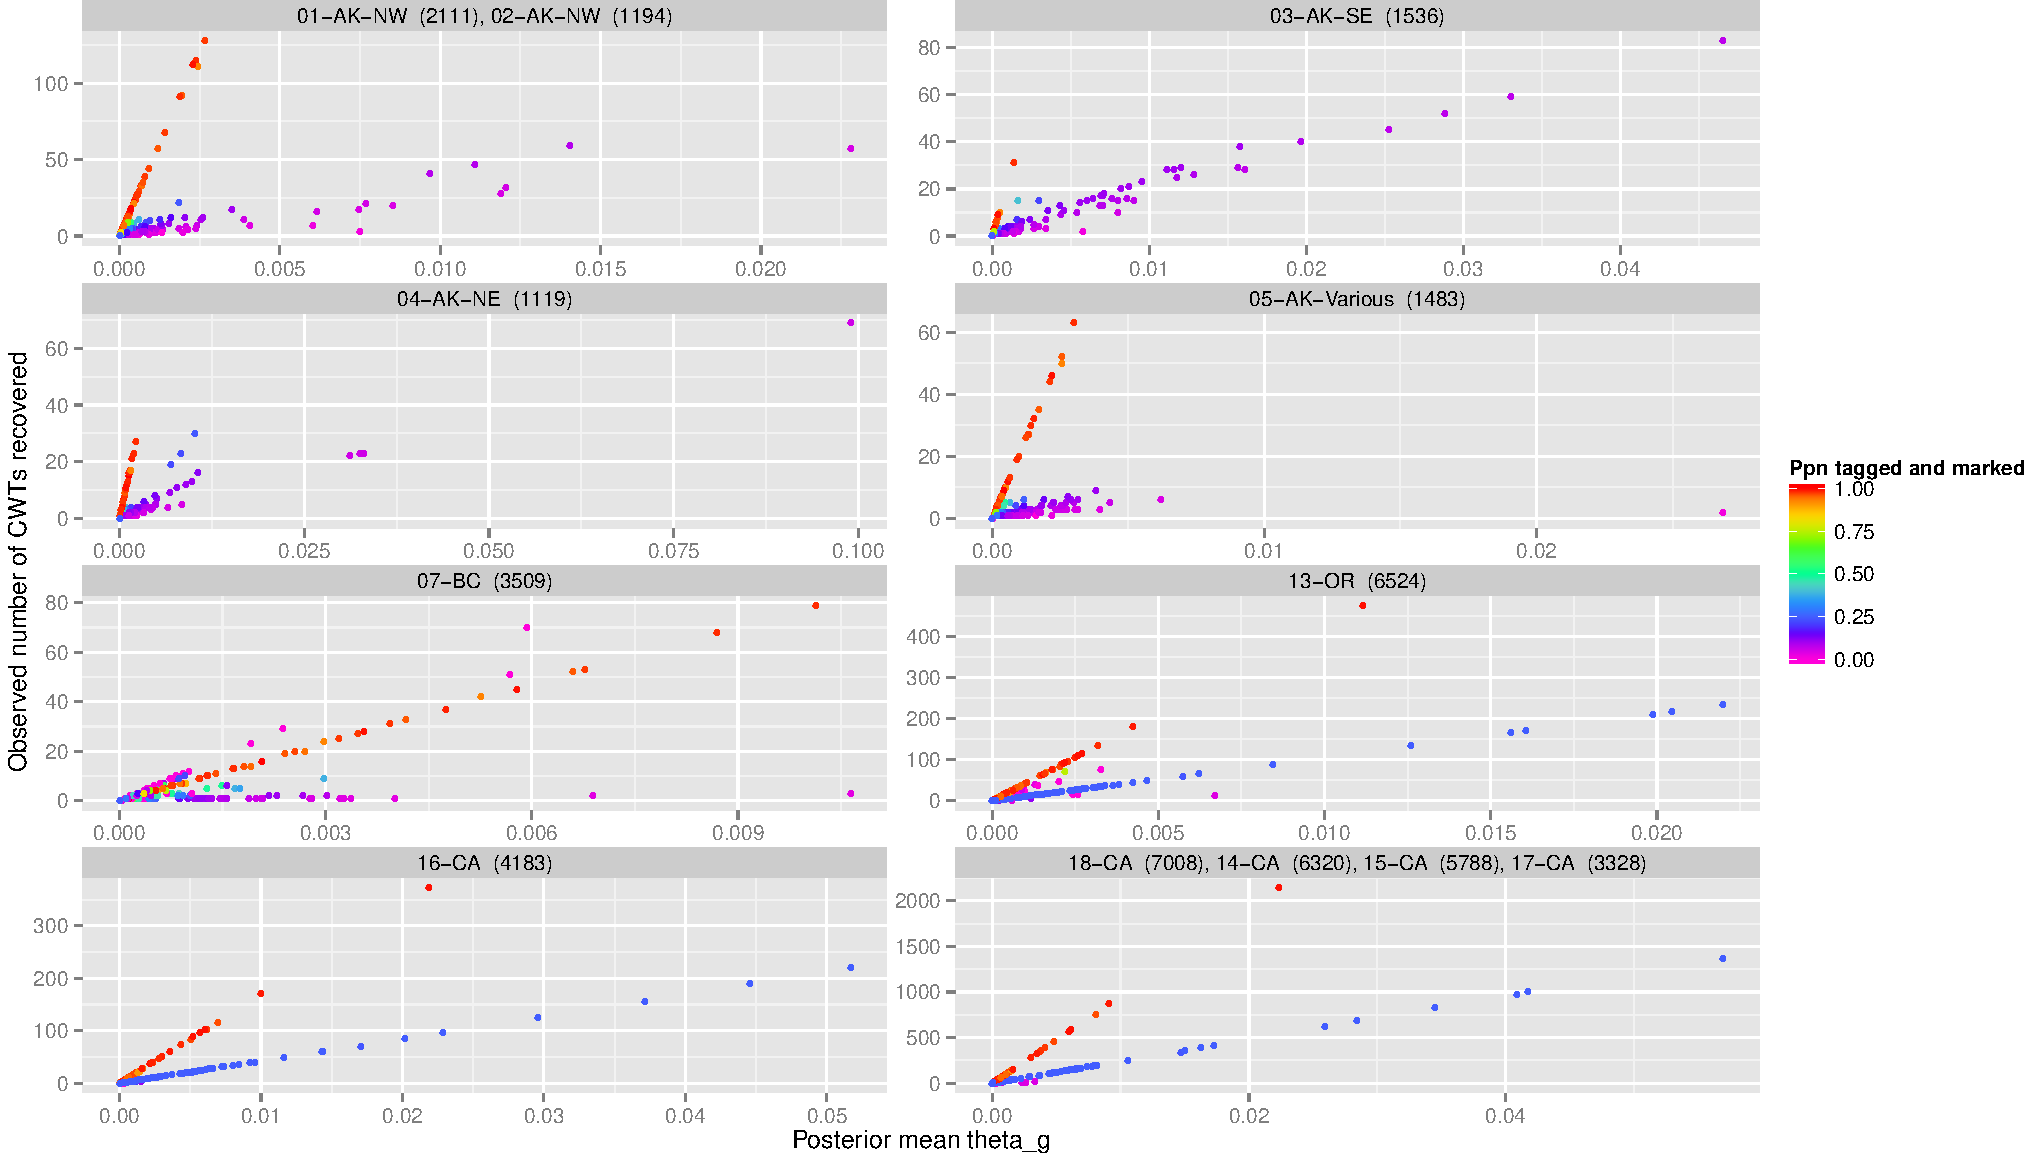
\includegraphics[width=\textwidth]{images/post_mean_theta_v_counts_f_marked_times_p_marked.pdf}
\end{center}
\caption{Posterior mean $\theta_g$ plotted on $x$-axis with observed number of CWTs recovered on $y$.  Each point is a
tag code colored by the proportion of the release group associated with the tag code that is both ad-clipped and tagged.}
\end{sidewaysfigure}



\section{Comparison of PBT to CWTs \label{sec:compare}}

Not yet done.

\bibliography{../bibstuff/pbtfeas}
\bibliographystyle{../bibstuff/men}
 \end{document}
